\documentclass[10pt,a4paper]{article}
\usepackage[T1]{fontenc}
\usepackage[utf8]{inputenc}
\usepackage[english]{babel}
\usepackage{amsmath,booktabs,geometry,graphicx,hyperref}
\geometry{margin=1.4cm}
\hypersetup{colorlinks=true,urlcolor=blue,linkcolor=blue}

\title{Lifted Successor Joins in a First-Order PDDL Planner:\\
An HTG VisitAll Case Study}
\author{Technical Report on \texttt{pddl\_fol}}
\date{September 25, 2026}

\begin{document}
\maketitle

\begin{abstract}
We test whether the small \texttt{folplan} planner can compete on a
hard-to-ground PDDL family. We replace complete Cartesian action grounding
with joins between necessary positive precondition atoms and the current
state, followed by full formula evaluation. On eight official five-dimensional
VisitAll instances, the previous version solves one within a 1 GiB limit;
the lifted version solves six. It beats the research-grade lifted planner
Powerlifted in full-process latency on four shallow instances, reaching
0.021 versus 0.118 seconds on \texttt{p8}. Powerlifted solves all eight and
is substantially faster on deeper tasks. The result identifies a useful
low-latency niche, not general planning competitiveness.
\end{abstract}

\section{Motivation and design}
Classical PDDL actions are schematic. Grounding all parameter tuples can
dominate planning even when only a few actions are applicable in each state.
Corr\^ea et al.\ describe lifted successor generation as conjunctive query
evaluation~\cite{correa2020}. The indexed \texttt{folplan} baseline still
grounded every typed parameter tuple before search~\cite{priorstudy}.

For each schema, our new generator collects positive atoms reached only
through conjunction in its precondition. It joins their arguments against
facts in the current state, binding action parameters, then enumerates any
unbound parameters over their declared object types. The full first-order
precondition is evaluated for every candidate. Disjunction, negation,
implication, and quantified subformulas contribute no join constraint;
schemas without a usable positive atom use bounded Cartesian fallback.
Candidates are ordered by schema and original object order, preserving the
breadth-first search tie break. At most 256 positive conjuncts enter the
join; the complete formula remains checked. The ground-action limit now
counts distinct candidates emitted across search states, before the full
formula test, rather than the full Cartesian universe.

The five-dimensional VisitAll move schemas each have six \texttt{pos}
parameters. They require one five-argument \texttt{at-robot} fact and one
\texttt{neighbor} pair. In a state with one robot location, these relations
bind almost every parameter before effects are applied. With 24 objects,
naive grounding would enumerate $5\cdot24^6=955{,}514{,}880$ actions.

\section{Experimental protocol}
We use official \texttt{5-dim-visitall-CLOSE-g1} instances
\texttt{p0--p5,p8,p9} from the HTG corpus at commit
\texttt{c5670ed2}~\cite{htg}.
These eight instances contain 6--24 position objects; their different
goals require 3--13 steps, so the horizontal axis is not a pure size
scaling curve. We compare the prior indexed \texttt{folplan}, lifted
\texttt{folplan}, Fast Downward 26.6+ at commit \texttt{9b81c7e} with
\texttt{astar(blind())}, and Powerlifted at commit \texttt{bf54e169}
using \texttt{alt-bfws1}, FF, Yannakakis joins, and unit costs. The latter
is a competitive lifted heuristic planner~\cite{powerlifted}.

All binaries use release builds on one AMD Ryzen 5 7640U machine running
Linux 7.2.5. Each run gets a 1 GiB address-space cap and a 15-second
process timeout. Both \texttt{folplan} versions use a 100{,}000-state and
1{,}000{,}000-ground-action setting, with the changed candidate-limit
meaning described above. Wall time includes process startup, parsing,
translation, and search. Solved results are medians of five interleaved
runs; a solver that hit a limit was recorded once per instance. Powerlifted's
Python driver is included in its full-process time. Raw measurements and
status codes are in \path{benchmarks/results/htg-visitall-raw.csv}; summary
data are in \path{benchmarks/results/htg-visitall-summary.csv}.
The command-line harness is \path{benchmarks/run_visitall.py}.

\section{Results}
\begin{table}[h]
\centering
\small
\begin{tabular}{lrrrrr}
\toprule
Instance & Objects & Steps & Indexed (s) & Lifted (s) & Powerlifted (s) \\
\midrule
\texttt{p0} & 6  & 4  & 0.333 & 0.051 & 0.119 \\
\texttt{p1} & 8  & 3  & G     & 0.012 & 0.118 \\
\texttt{p2} & 10 & 5  & G     & 0.388 & 0.145 \\
\texttt{p3} & 12 & 6  & G     & M     & 0.143 \\
\texttt{p4} & 14 & 5  & G     & 1.443 & 0.123 \\
\texttt{p5} & 16 & 3  & G     & 0.043 & 0.117 \\
\texttt{p8} & 22 & 3  & G     & 0.021 & 0.118 \\
\texttt{p9} & 24 & 13 & G     & M     & 1.878 \\
\bottomrule
\end{tabular}
\caption{Median full-process seconds. G: ground-action cap; M: 1 GiB memory
cap. Fast Downward solved only \texttt{p0} (9.138 s); its translator hit the
memory cap on all other instances.}
\label{tab:results}
\end{table}

\begin{figure}[h]
\centering
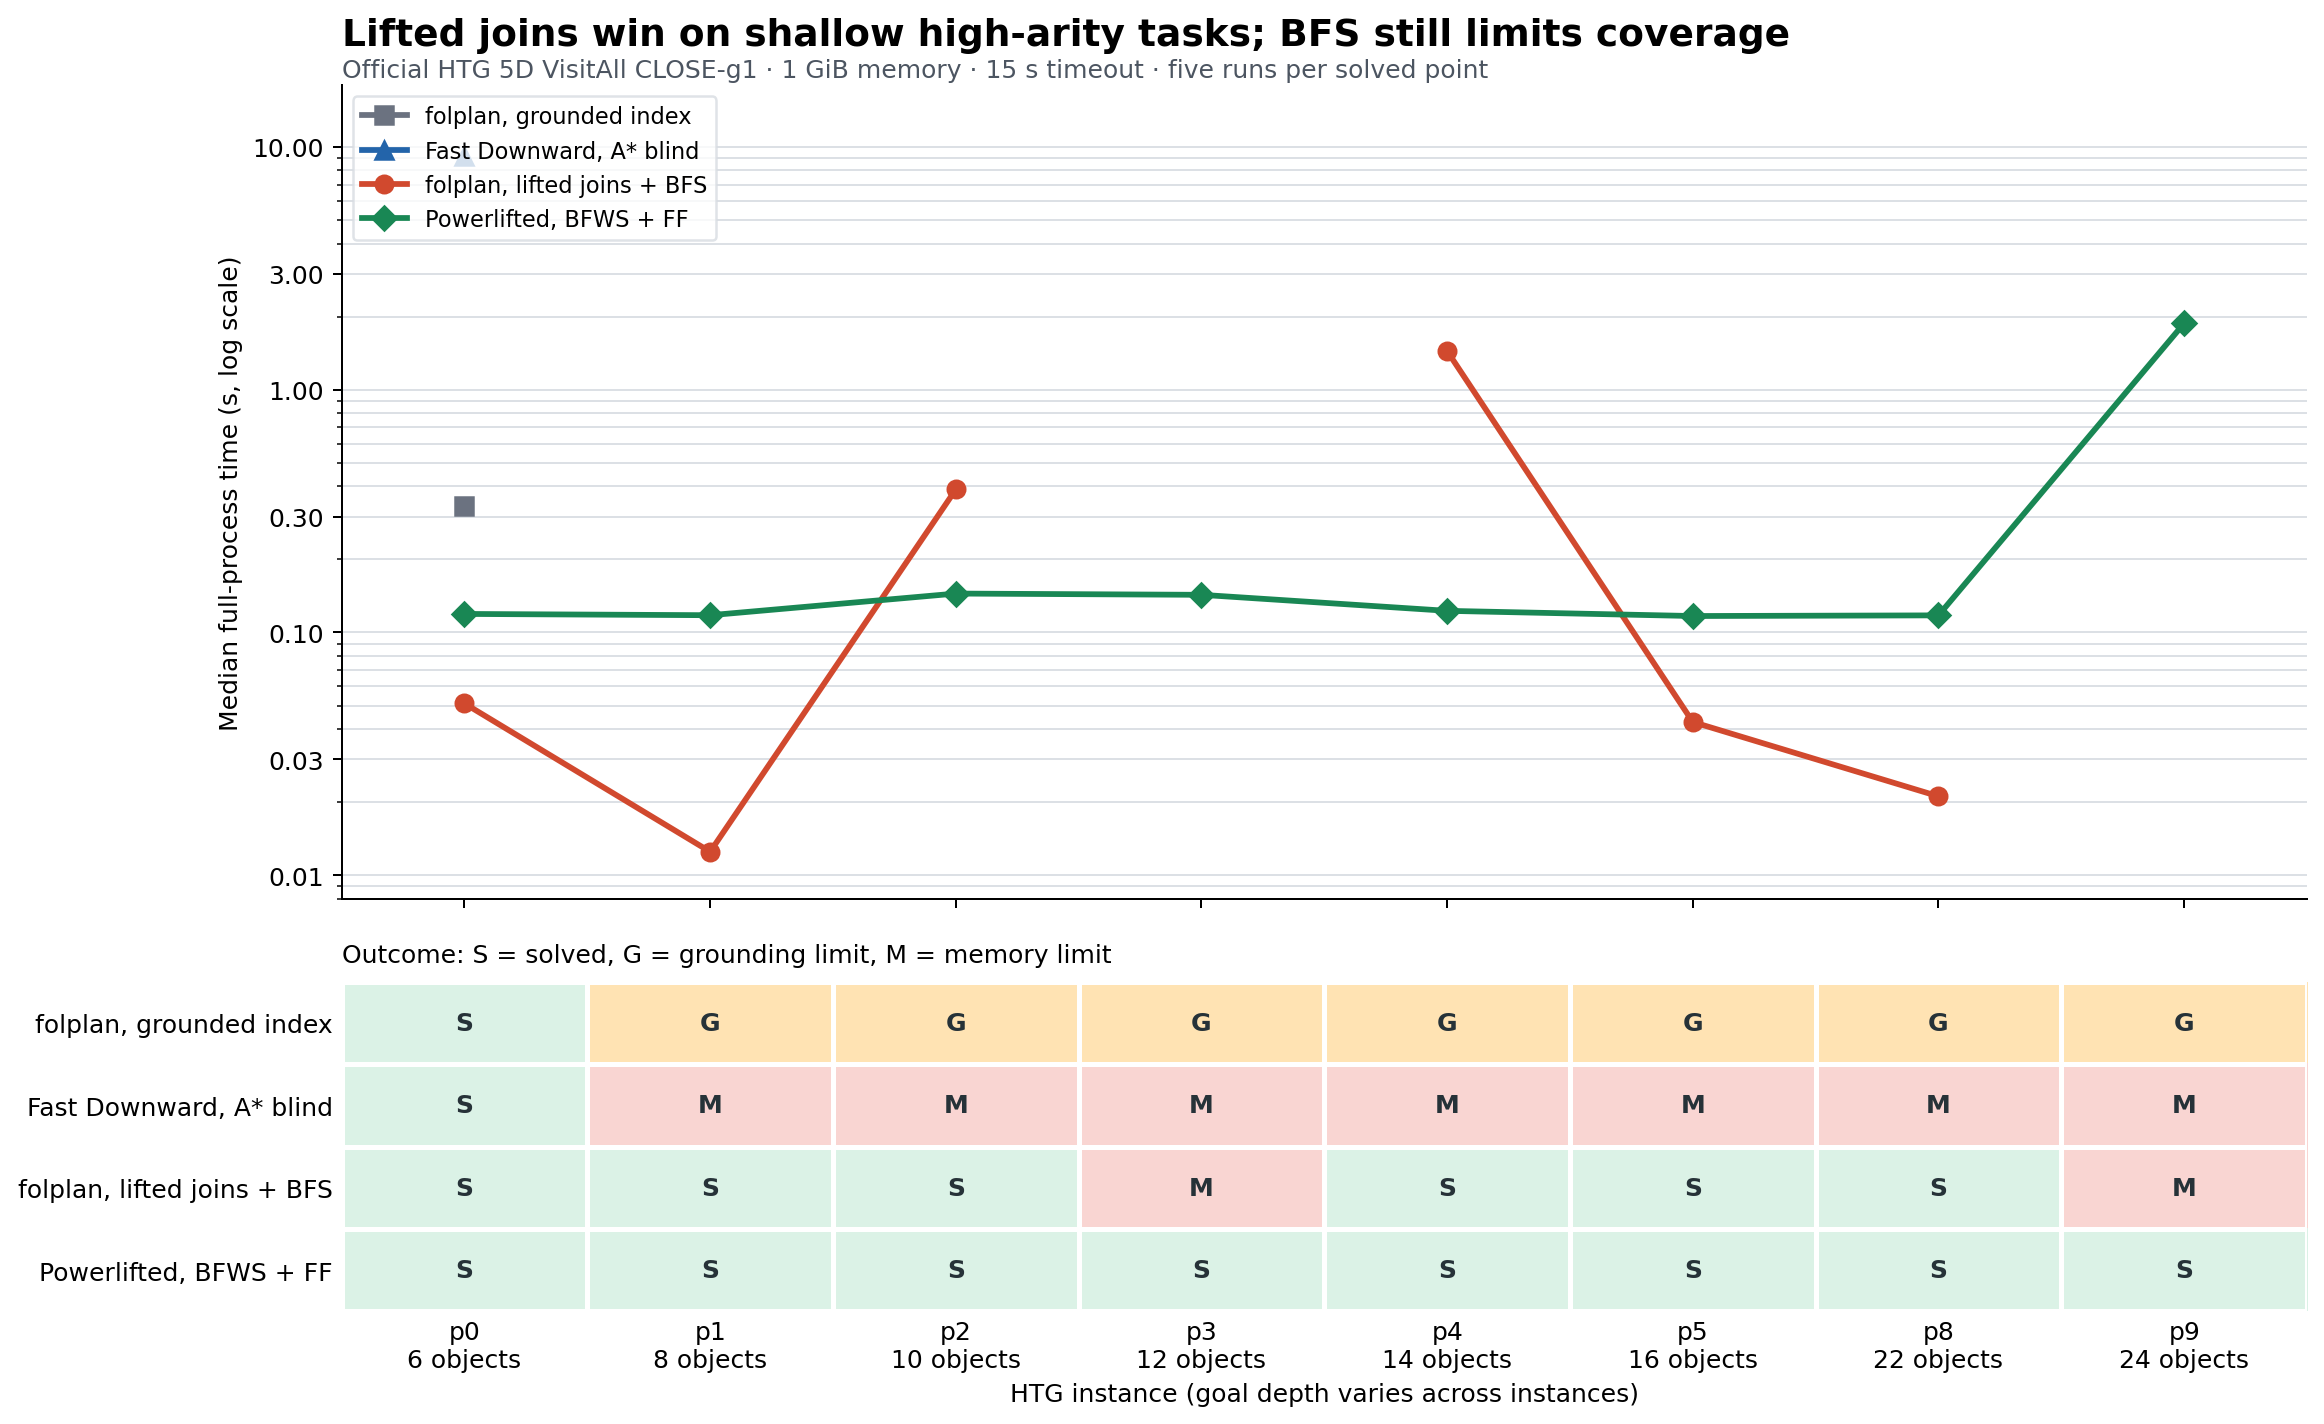
\includegraphics[width=0.80\linewidth]{figures/htg-visitall-performance.png}
\caption{Runtime of solved cases and outcome of all four planners. Gaps in
runtime lines mark unsolved cases; goal depth varies between instances.}
\label{fig:results}
\end{figure}

Lifted joins remove the immediate grounding failure: \texttt{p1} has
$5\cdot8^6=1{,}310{,}720$ raw action tuples, already above the baseline's
cap. On \texttt{p8}, the lifted planner is $5.57\times$ faster than
Powerlifted in full-process time; on \texttt{p1}, $9.43\times$ faster.
This advantage is chiefly startup latency, not faster search: Powerlifted
reports roughly 0.002 seconds of internal search on \texttt{p8}, while its
full process takes 0.118 seconds. It expands only three states, versus
74 states explored by our breadth-first search.

At five or more steps, search dominates. Powerlifted is $2.68\times$
faster on \texttt{p2} and $11.75\times$ faster on \texttt{p4}; lifted
\texttt{folplan} reaches the memory cap on \texttt{p3} and \texttt{p9}.
All reported solved cases have matching plan lengths, but Powerlifted's
configuration does not in general guarantee optimality. The results
suggest that heuristic guidance and a more compact state representation,
not more grounding work, are the next bottlenecks.

\section{Limits and conclusion}
This is one PDDL family, eight selected instances, one host, and one
configuration per competitor. \texttt{astar(blind())} isolates a grounded
Fast Downward baseline rather than its strongest heuristic portfolio.
Comparisons between a Rust CLI and Powerlifted's Python driver measure
deployment latency as well as planning work. The old and new
\texttt{max-ground-actions} settings bound different quantities.
Thus four latency wins establish a narrow use case for lifted joins,
while Powerlifted's full coverage shows that the planner is not yet
competitive on the harder part of this family.

\small
\begin{thebibliography}{9}
\bibitem{correa2020}
A.~B. Corr\^ea, F. Pommerening, M. Helmert, and G. Franc\`es,
"Lifted Successor Generation Using Query Optimization Techniques,"
\emph{ICAPS}, vol. 30, pp. 80--89, 2020.
\url{https://doi.org/10.1609/icaps.v30i1.6648}.
\bibitem{powerlifted}
A.~B. Corr\^ea and J. Seipp,
"Best-First Width Search for Lifted Classical Planning,"
\emph{ICAPS}, vol. 32, pp. 11--15, 2022.
\url{https://doi.org/10.1609/icaps.v32i1.19780}.
\bibitem{htg}
A.~B. Corr\^ea, \emph{htg-domains}, corpus commit \texttt{c5670ed2}.
\url{https://github.com/abcorrea/htg-domains/tree/c5670ed289f58d3d6e104d7b06f311cf2f87b354}.
\bibitem{priorstudy}
\texttt{pddl\_fol}, "Indexing Necessary Preconditions for PDDL
Successor Generation," technical report, 2026.
\path{docs/successor-index-study.tex}.
\end{thebibliography}
\end{document}
